% ==============================================================================
% ================================== AUFGABE 3 ================================
% ==============================================================================

\section{Aufgabe 3: Analyse des Treibstoff-Features}
\label{sec:aufgabe3}

\subsection{Methodik}

Die Analyse aus Aufgabe~\ref{sec:aufgabe1} wird um das Feature \texttt{fuel\_episode} erweitert. Neben der Pearson- und Spearman-Korrelation werden die Episoden in Quartile des Treibstoffverbrauchs eingeteilt und der mittlere Reward pro Quartil verglichen. Ergänzend wird die kombinierte Verteilung von Länge und Treibstoff farbcodiert nach Reward dargestellt. Die methodische Grundlage der Korrelationsanalyse folgt Géron \cite[S.~109--112]{1} sowie den in Aufgabe~\ref{sec:aufgabe1} dargestellten Verfahren.

\subsection{Ergebnisse}

Die Quartilsanalyse zeigt einen klaren Aufwärtstrend: Q1 (niedrigster Verbrauch) erzielt im Mittel $275{,}28$, Q2 $270{,}47$, Q3 $289{,}66$ und Q4 (höchster Verbrauch) $291{,}56$ (eigene Messung). Die Korrelation zwischen Länge und Treibstoff beträgt $r = 0{,}474$.

\begin{figure}[H]
    \centering
    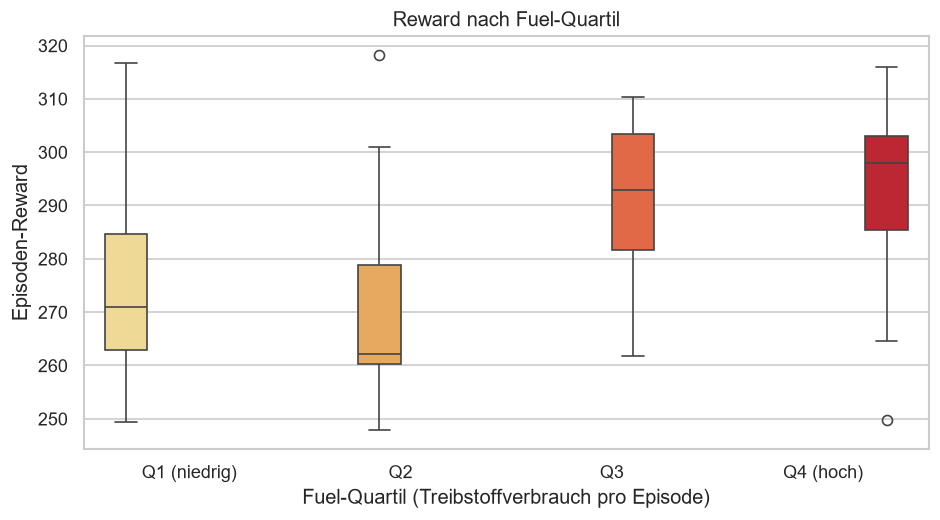
\includegraphics[width=0.9\linewidth]{asset/image/TomaKing_A3_Reward_nach_Fuel_Quartil.png}
    \caption{Reward nach Treibstoff-Quartil \textit{(eigene Darstellung)}.}
    \label{fig:a3_quartile}
\end{figure}

\begin{figure}[H]
    \centering
    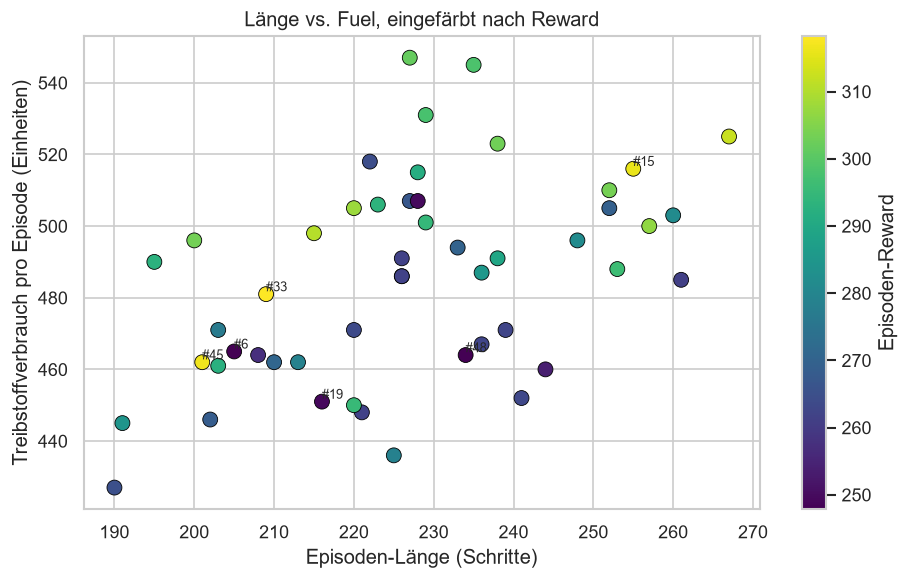
\includegraphics[width=0.9\linewidth]{asset/image/TomaKing_A3_Laenge_vs_Fuel.png}
    \caption{Länge vs.\ Treibstoff, farbcodiert nach Reward \textit{(eigene Darstellung)}.}
    \label{fig:a3_combined}
\end{figure}

\subsection{Interpretation}

Erwartungswidrig korreliert der Treibstoffverbrauch positiv mit dem Reward. Wie in Aufgabe~\ref{sec:aufgabe2} diskutiert, ist dieser Zusammenhang als Selection-Bias zu interpretieren: Episoden mit hohem Verbrauch sind jene, in denen der Agent aktiv korrigiert und präzise landet. Die Quartilsanalyse (Abbildung~\ref{fig:a3_quartile}) zeigt den Zusammenhang robuster als eine einzelne Korrelation, weil Ausreißer weniger stark wirken (eigene Interpretation auf Basis der Quartilsanalyse).

% ==============================================================================
% ================================== AUFGABE 3 ================================
% ==============================================================================